\chapter{Online Adaptation}
\label{chap:adaptation}
%\url{https://github.com/clab/fast_align}
In this chapter, we experiment we online adaptation of the proposed enhanced ASR pipeline.

We assume that a speaker does many errors systematically, for example due his/her native language. We expect, some of these errors can be identified and corrected in the ASR phoneme-to-grapheme translation model. We plan to identify this corrections and extract simple rewriting rules. These rewriting rules would be applied prior to feeding them into the ASR/SLT translation model in the pipeline.

\XXX{chapter organization}

\section{Enhanced ASR/SLT Pipeline with Online Adaptation}
\label{oeasr:model}
We propose the enhanced ASR pipeline with online adaptation as follows: the acoustic model outputs the phoneme transcripts. The phoneme transcripts are adapted using the Online Adaptation model. The adapted output (still in phonemes) is fed into the phoneme-to-grapheme translation model. The translation model translate the phoneme input into graphemes using beam search. The model outputs the best translation candidate from the beam as translation of the whole ASR pipeline. All beam translations are passed through the \texttt{phonemizer} and the online adaptation model learns new rules from the transcripts.

In the case of SLT pipeline, two phoneme-to-grapheme translation models are needed: the ASR and the SLT. The ASR translation model would be used for obtaining ``traning data'' for the online adaptation model.

The schema of the proposed enhanced ASR pipeline with online adaptation is in \cref{fig:online_easr}.

\begin{figure}[t]
	\centering
	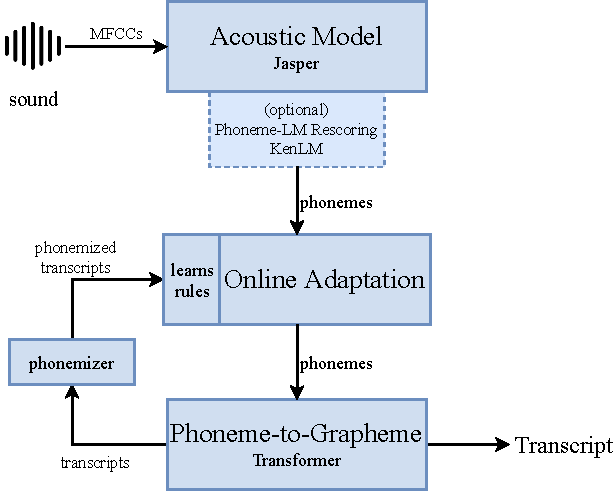
\includegraphics[width=.9\textwidth]{img/online_easr}
	\caption{Enhanced ASR pipeline with online adaptation.}
	\label{fig:online_easr}
\end{figure} 


\subsection{Online Adaptation Model}
The obvious requirement on the online adaptation model is that it must be able to learn quickly. Hence, we rule out neural networks as they require higher volume of training data. If not provided, the neural networks tend to over-fit the examples. 

Therefore, we decided for rule-based model. We take our inspiration in work we previously reviewed for phoneme-to-grapheme models (see \cref{easr:rel_asr}). More precisely, the work of \perscite{horndasch2006phoneme}. Their main objective is to find appropriate orthographic representations for phoneme strings. Our use case differs as we seek phoneme-to-phoneme mapping correcting errors instead of phoneme-to-grapheme mapping. Using a expectation-maximization algorithm \parcite{dempster1977maximum}, we seek the best ``correct-to-incorrect'' phoneme alignment (in their setup, they are looking for best phoneme-to-grapheme alignment). In the second step, we cluster neighboring symbols together to account for the insertions (i.e., to remove ``$\epsilon$ to phoneme'' rules). Finally, $n$-gram probabilities of symbol pairs are learned. During the inference, the input string is split into individual symbols. For each symbol are generated all possible symbol pairs. According to the beam width, the best sequences are taken. 

\paragraph{Model Training}
As already described, we learn the phoneme rewrite rules from aligned ``incorrect-to-correct'' phoneme transcriptions. To align these transcriptions, we utilize expectation-maximization algorithm as follows:

\begin{enumerate}
	\item Compute the initial \texttt{alignment} using modified Levenstein distance algorithm (insertion, deletion and substitution operations are considered, each with the same cost).
	
	\item \emph{While} substitution frequencies change do:
	\begin{enumerate}
		\litem{Expectation step:} based on the \texttt{alignment}, compute the substitution frequencies,
		
		\litem{Maximization step:} align training pairs  based on frequencies using dynamic programming.
	\end{enumerate}
\end{enumerate}

The last computed alignment defines the rewrite rules: ``rewrite the symbol from the source string (the ``incorrect'' one) to the symbol on the corresponding position in the target string (the ``correct'' one)''. The insertions in the alignment are represented with special $\epsilon$ character in the source string (insertion, \textipa{Ins3:S@n}):

\begin{center}
	\begin{tabular}{c}
		\textipa{Ins3:}\large{$\epsilon\epsilon\epsilon$}  \\
		\textipa{Ins3:}\large{\textipa{S@n}}
	\end{tabular}
\end{center}

 We do not allow rules ``$\epsilon \rightarrow \dots$'', because they do not have straightforward representation during the beam search decoding. Instead, we cluster the rules with $\epsilon$ symbol as head with neighbors using following algorithm:
   
\begin{enumerate}
	\item For each \texttt{rule} in \texttt{alignment}:
	\begin{enumerate}
		\item If \texttt{rule} is \emph{empty}: join with previous or next; \texttt{rule}
		\item Else: add to \texttt{new\_rules}.
	\end{enumerate}
\end{enumerate}

From the above insertion example, we would extract following rewrite rules:

\begin{center}
	\begin{tabular}{c|c|c|c}
		\textipa{I} $\rightarrow$ \textipa{I} &
		\textipa{n} $\rightarrow$ \textipa{n} &
		\textipa{s} $\rightarrow$ \textipa{s} &
		\textipa{3:} $\rightarrow$ \textipa{3:S@n}.
	\end{tabular}
\end{center}

Finally, we train an $n$-gram model. The function of the $n$-gram model is to learn interactions between the neighboring phoneme rewriting rules. We utilize the KenLM for this task. As the KenLM is word-oriented, we dump the rules as separate words in form ``source-target''. We substitute the space symbol with underscore.

\paragraph{Inference}
We use the trained $n$-gram model during the inference --- rewriting input using the rules. For this, we utilize beam search:

\begin{enumerate}
	\item For each symbol from the input:
		\begin{enumerate}
			\item generate candidates using rules with corresponding source symbol,
			\item score the candidates using the $n$-gram model,
			\item keep top $w$ candidates according to the beam width $w$. 
		\end{enumerate}
\end{enumerate}



\section{Experiments}
\label{oeasr:experiments}
In this section, we experiment with different variations of the proposed online adaptation algorithm.

For testing of the adaptation model, we use the parallel Czech - English ASR/SLT test set \texttt{read-newstest} (see \cref{read-newstest} on page \pageref{read-newstest}). To develop the adaptation model independently on the phoneme-to-grapheme model, we use instead of corrected transcripts that would be given by the P2G model the golden transcripts. Additionally, we create ``fake'' acoustic output with artificial errors to better analyze the behavior of the model.

We simulate ``online'' online adaptation by iterating over the test set with step of 100 sentences, i.e., we in each iteration the training set for the adaptation model grows by 100 sentences and the model corrects next 100 sentences.

\subsection{Na\"ive Approach: Train \& Rewrite All}
We first experiment with a rather ``na\"ive'' approach --- we use all sequences for training of the adaptation model and we rewrite all phoneme transcripts flowing through the model (i.e., disregarding correctness of the substrings/words). This means, that we create \emph{identity} rewrite rules even for correct words (e.g., ``\textipa{@} $\rightarrow$ \textipa{@}'') and the $n$-gram model teaches on all this rules. 

Our motivation to test this approach is that we assume that the speaker makes errors systematically (e.g., instead of [\textipa{nt}] pronounces [\textipa{nd}] in every word).

\paragraph{Test on artificial data}
In order to have better control, we first test this na\"ive method on artificial data. We take the golden phoneme transcripts of the English \texttt{read-news\-test} and introduce errors to it. We decided to start with one systematic error of the speaker: to pronounce [\textipa{nt}] as [\textipa{nd}]. 

We set the order of the $n$-gram model to 2 (the smallest allowed order) and simulate the adaptation. 

During the first step (first 100 sentences are used for training, following 100 sentences for correction) we dump the obtained rules: We get identity rules for each phoneme except for ``\textipa{t}'' for which we have two rules (``\textipa{t} $\rightarrow$ \textipa{t}'' and ``\textipa{t} $\rightarrow$ \textipa{d}''). This is as expected. 

Now we want the $n$-gram model to ``learn'' that this rule is applied only for phoneme pair [\textipa{nd}].

We take a closer look at the $n$-gram training data. We calculate following 2-gram probabilities:

\begin{equation}\label{rule1}
	P( \textnormal{\textipa{d} $\rightarrow$ \textipa{d}} | \textnormal{\textipa{n} $\rightarrow$ \textipa{n}}) =
	\frac{
		c( \textnormal{\textipa{d} $\rightarrow$ \textipa{d}} | \textnormal{\textipa{n} $\rightarrow$ \textipa{n}})
	}{
		\sum\limits_{r \in \textnormal{Rules}} c( r | \textnormal{\textipa{n} $\rightarrow$ \textipa{n}})
	} =
	\frac{82}{398},
\end{equation}

\begin{equation}\label{rule2}
P( \textnormal{\textipa{d} $\rightarrow$ \textipa{t}} | \textnormal{\textipa{n} $\rightarrow$ \textipa{n}}) =
\frac{
	c( \textnormal{\textipa{d} $\rightarrow$ \textipa{t}} | \textnormal{\textipa{n} $\rightarrow$ \textipa{n}})
}{
	\sum\limits_{r \in \textnormal{Rules}} c( r | \textnormal{\textipa{n} $\rightarrow$ \textipa{n}})
} =
\frac{61}{398},
\end{equation}

\begin{equation}
\forall r \in \textnormal{Rules}, r \neq \textnormal{\textipa{n} $\rightarrow$ \textipa{n}}: P( \textnormal{\textipa{d} $\rightarrow$ \textipa{t}} | r) = 0.
\end{equation}
%-49.90927171707153 -54.84227800369263

We also check the probabilities given by the KenLM. For both rewrite rules \cref{rule1,rule2}, the KenLM outputs equal probabilities, which is incorrect. We assume, this may be due to lower precision that is needed when working with large amounts of data, which is not our case. To overcome this, we implement our own $n$-gram model and continue in analysis.

In case of extending string ``\textipa{tSEk mEn \ae n}'' (Czech men an[d]), the beam search (BS) correctly applies both rules creating two beams. The beam with suffix ``\textipa{d}'' has higher probability.

A problem emerges when the BS further extends the beams and comes to point ``\textipa{tSEk mEn \ae nd wImIn \ae \*r9n}'' (Czech men and women aren'[t]). Again, the BS correctly applies both rules, producing beams ``\textipa{tSEk mEn \ae nd wImIn \ae \*r9nd}'' and ``\textipa{tSEk mEn \ae nd wImIn \ae \*r9nt}''. The latter is correct, but the former has higher probability as the 2-gram ``\textipa{n} $\rightarrow$ \textipa{n} \textipa{d} $\rightarrow$ \textipa{d}'' has higher probability.

\begin{figure}[h]
	\includegraphics[width=\linewidth,height=5cm]{img/naive}
	\caption{Naive adaptation on artificial data ([\textipa{nt}] replaced with [\textipa{nd}]). WER of 100 subsequent sentences rewritten using rules obtained from all previous sentences.}
	\label{fig:naive} 
\end{figure}

\begin{figure}[h]
	\includegraphics[width=\linewidth,height=5cm]{img/naive_english}
	\caption{Naive adaptation on English \texttt{read-newstest} outputted by the acoustic model. WER of 100 subsequent sentences rewritten using rules obtained from all previous sentences.}
	\label{fig:naive_en} 
\end{figure}

One way, how to minimize the occurrence of this error is to higher the order of the $n$-gram model. In \cref{fig:naive}, we can observe a clear advantage of the higher-order models over the lower ones.

The na\"ive approach fails on real data outputted by the acoustic model. We witness quite substantial deterioration of the performance compared to the non-adapted source in \cref{fig:naive_en}.

\subsection[Revised Na\"ive Approach: Train \& Rewrite All Word-by-Word]{Revised Na\"ive Approach: Train \& Rewrite All \\Word-by-Word}


\begin{figure}[h]
	\includegraphics[width=\linewidth,height=7cm]{img/naive_revised}
	\caption{}
	\label{fig:naive_revised} 
\end{figure}

\begin{figure}[h]
	\includegraphics[width=\linewidth,height=7cm]{img/naive_revised_english}
	\caption{}
	\label{fig:naive_revised_en} 
\end{figure}

sequence labeling

